%%%%%%%%%%%%%%%%%%%%%%%%%%%%%%%%%%%%%%%%%%%%%%%%%%%%%%%%%%%%%%%%%%%%%%%%%%%%%%%%
%%%%%%%%%%%%%%%%%%%%%%%%%%%%%%%%%%%%%%%%%%%%%%%%%%%%%%%%%%%%%%%%%%%%%%%%%%%%%%%%
%%                          AUTHOR: BIBEKANANDA DATTA                         %%
%%                             (C) SEPTEMBER 2023                             %%
%%                      PhD STUDENT, MECHANICAL ENGINEERING                   %%
%%                           JOHNS HOPKINS UNIVERSITY                         %%
%%%%%%%%%%%%%%%%%%%%%%%%%%%%%%%%%%%%%%%%%%%%%%%%%%%%%%%%%%%%%%%%%%%%%%%%%%%%%%%%
%%%%%%%%%%%%%%%%%%%%%%%%%%%%%%%%%%%%%%%%%%%%%%%%%%%%%%%%%%%%%%%%%%%%%%%%%%%%%%%%
%%             PLEASE CHECK THE README.md FILE BEFORE YOU PROCEED             %%
%%              it may be conveneint to read this file on GitHub              %%
% https://github.com/bibekananda-datta/JH-MechE-Dissertation-Proposal-Template %
%% template hosted on the GitHub repository is likely to be the most updated  %%
%%%%%%%%%%%%%%%%%%%%%%%%%%%%%%%%%%%%%%%%%%%%%%%%%%%%%%%%%%%%%%%%%%%%%%%%%%%%%%%%


%%%%%%%%%%%%%%%%%%%%%%%%%%%%%%%%%%%%%%%%%%%%%%%%%%%%%%%%%%%%%%%%%%%%%%%%%%%%%%%%
% this is an unofficial template for the thesis or dissertation proposal in 
% the Department of Mechanical Engineering at Johns Hopkins University. 
% consult with the department or advisor before using the template.
% this template includes comments on the department-suggested page limits. 
% however, it is the user's responsibility to ensure the formatting conforms 
% with the advisor or proposal committee or department's requirement.
% this template is based on the LaTeX article class and uses BibLaTeX as 
% bibliographic manager. Use a citation manager to generate the BibLaTeX file.
%%%%%%%%%%%%%%%%%%%%%%%%%%%%%%%%%%%%%%%%%%%%%%%%%%%%%%%%%%%%%%%%%%%%%%%%%%%%%%%%



%%%%%%%%%%%%%%%%%%%%%%%%%%%%%%%%%%%%%%%%%%%%%%%%%%%%%%%%%%%%%%%%%%%%%%%%%%%%%%%%
%% if possible, please make your formatting changes here through the variables 
%% go through all the variables and understand what role they play in formatting
%%%%%%%%%%%%%%%%%%%%%% LIST OF VARIABLES FOR FORMATTING %%%%%%%%%%%%%%%%%%%%%%%%

\def\FontPackage{lmodern}                   % latin modern font (you can also change it to times)
\def\BibFileName{references.bib}            % name of BibLaTeX file with all the bibliography

\def\NoSectionLevel{3}                      % 3 levels for sections ... to subsubsection
\def\TocIndent{0}                           % indentation in the list of figs and tables
\def\NoTocLevel{3}                          % no of levels showed in the table of contents
%% 3 levels mean section to subsubsection.. decrease if you want less to showup in TOC

% font format for section heading and title
\def\SectionFont{\large\bfseries}           % section heading font format
\def\SubsectionFont{\normalsize\bfseries}   % subsection heading font format
\def\SubsubsectionFont{\normalsize\itshape} % subsubsection heading font format
\def\CaptionFontSize{small}                 % caption font size
\def\CaptionFontType{bf}                    % boldface label for captions
\def\CaptionSeparator{colon}                % separates caption heading from text. can use 'period' as well

%% if this seems too widespread for you, try changing it locally using
%% \begin{group} ... \renewcommand{\arraystretch} ... \end{group} commands
\def\GlobalTableSpacing{1.2}                % global spacing parameter for table

\def\ParagraphSpacing{\baselineskip}        % spacing between paragraph
\def\ParagraphIndent{0}                     % indentation at the beginning of the paragraph
\def\FullCiteSpacing{1.1}                   % spacing in a fullcite item
\def\BibItemSpacing{0.5\baselineskip}       % spacing between bibliographic items in reference
\def\FootnoteSpacing{0.5\baselineskip}      % spacing between footnotes
\def\CaptionSpacing{0}                      % spacing between the figure and the caption (unit: pt)

%%%%%%%%%%%%%%%%%%%% END LIST OF VARIABLES FOR FORMATTING %%%%%%%%%%%%%%%%%%%%%%




%%%%%%%%%%%%%%%%%%%%%%%%%%%%%%%%%%%%%%%%%%%%%%%%%%%%%%%%%%%%%%%%%%%%%%%%%%%%%%%%
%% add packages as needed but sometimes the order of the packages matter.
%% I primarily tried to load the packages in alphabetical order unless or 
%% based on their functionalities (all math/ table packages) unless there 
%% is an issue with dependency, then I included packages in that order.
%% you may get warning/ error for the order in which packages are included
%% you may have to change the options in biblatex package for bibliography
%%%%%%%%%%%%%%%%%%%%%%%%%%% LaTeX CLASS AND PACKAGES %%%%%%%%%%%%%%%%%%%%%%%%%%%

\documentclass[12pt]{article}               % document class (article - 12 pt)

\usepackage[utf8]{inputenc}	                % for encoding input character
\usepackage[pagewise,mathlines]{lineno}     % linenumbers


%% math packages
\usepackage{amsfonts,amssymb,amsmath,amsthm,autobreak,cancel,dsfont,mathtools,mathbbol,mathrsfs,siunitx,upgreek}

\usepackage[ruled]{algorithm2e}             % to manage algorithm environment
\usepackage[titletoc]{appendix}             % to manage appendix chapters
\usepackage[american]{babel}                % for different language typography

%% bibliographic package (make sure your bib file is in BibLaTeX format)
%% use Zotero or some other reference manager to generate the BibLaTeX file
%% change the style or other options if you need to
\usepackage[backend=biber, style=nature, maxnames=9, date=year, isbn=false, url=false, doi=true]{biblatex}
% \usepackage[backend=biber, style=apa, isbn=false, url=false, doi=true]{biblatex}

\usepackage{blindtext}                      % to generate random filler texts
\usepackage{calc}                           % to set arithmetic arguments for spacing
\usepackage{caption}                        % to manage captions
\usepackage{color}                          % color related packages
\usepackage{csquotes,epigraph,varwidth}     % for managing quotes
\usepackage{enumitem}                       % to manage list environment
\usepackage{float}                          % to manage floating environment
\usepackage[T1]{fontenc}                    % for font encoding
\usepackage[bottom]{footmisc}               % footnote environment management
\usepackage{graphicx,wrapfig}               % to manage images
\usepackage{geometry}                       % to manage margins and others
\usepackage{fancyhdr}                       % for header/ footer settings
\usepackage[dvipsnames]{xcolor}
\usepackage[a-1b]{pdfx}                     % to generate PDF/A file (before hyperref)
\usepackage[pdfa]{hyperref}                 % for hyperlinks
\usepackage[all]{hypcap}                    % for captions on the side of figures
\usepackage{ifthen}                         % if-then statement in algorithm
\usepackage{lscape}                         % landscape mode
\usepackage{listings}                       % to include codes

%% table related packages
\usepackage{booktabs,longtable,makecell,multicol,multirow,tabularx,xltabular}

\usepackage{parskip}                        % paragraph spacing 
\usepackage{setspace}                       % sets space between lines
\usepackage{seqsplit}                       % splits long character sequence
\usepackage[rightcaption]{sidecap}          % for sideway captions
\usepackage{tocbasic}                       % to manage table of contents
\usepackage{titlesec}                       % managing different titles
\usepackage{tikz}                           % package for drawing
\usepackage{subcaption}                     % individual panel and caption

%% add more packages and options as you need

%%%%%%%%%%%%%%%%%%%%%%%%% END LaTeX CLASS AND PACKAGES %%%%%%%%%%%%%%%%%%%%%%%%%



%%%%%%%%%%%%%%%%%%%%%%%%%%%%% DOCUMENT FORMATTING %%%%%%%%%%%%%%%%%%%%%%%%%%%%%%

%%% choice a font form (or add something else) for your thesis (uncomment one option)
\usepackage{\FontPackage}       
% if you want to use Palatino font, use the following and comment above line
%\usepackage[sc]{mathpazo}                  % palatino font family


%%% I use Zotero to generate the BibLaTeX file and include it in the same directory
\addbibresource{\BibFileName}


%%% margin settings with geometry package
\geometry{left=1.0in, right=1.0in, top=1.0in, bottom=1.0in}


%%% settings for the hyperref package
\hypersetup{linktocpage, unicode, colorlinks=true, citecolor=blue, filecolor=blue, linkcolor=blue, urlcolor=blue}
\urlstyle{rm}   % to remove the default URL style (tt format)


%%% settings for figure caption
\captionsetup{belowskip=\CaptionSpacing pt, font=\CaptionFontSize, labelfont=\CaptionFontType, labelsep=\CaptionSeparator, hypcap=true} 


%%% table of content, list of table, list of figure header setting with tocbasic
\addtotoclist[\jobname]{toc}
\renewcommand \tableofcontents{\listoftoc[{\contentsname}]{toc}}
\renewcommand*{\listoffigures}{\listoftoc[\listfigurename]{lof}}
\renewcommand*{\listoftables}{\listoftoc[\listtablename]{lot}}
\setuptoc{lof}{totoc}
\setuptoc{lot}{totoc}


%%% section, subsection, and subsubsection to appear in the TOC
\setcounter{secnumdepth}{\NoSectionLevel}


%%%% font and style for the section, subsection, subsubsection, etc.
\titleformat{\section}
{\SectionFont}{\thesection}{1em}{}[{\titlerule}]
\titleformat*{\subsection}{\SubsectionFont}
\titleformat*{\subsubsection}{\SubsubsectionFont}


%%%% paragraph, footnote, bib item, and table spacing
\setlength{\parskip}{\ParagraphSpacing}     % paragraph spacing
\setlength{\parindent}{\ParagraphIndent pt} % paragraph indentation
\setlength{\footnotesep}{\FootnoteSpacing}  % footnote separation
\setlength{\bibitemsep}{\BibItemSpacing}    % bib item separation 
\def\arraystretch{\GlobalTableSpacing}      % spacing in table


%%% settings for bibliography
\AtBeginBibliography{\urlstyle{rm}}
\DeclareFieldFormat{titlecase}{\MakeSentenceCase*{#1}}
\DeclareBibliographyCategory{fullcited}
\newcommand{\mybibexclude}[1]{\addtocategory{fullcited}{#1}}


%% settings for TikZ library (add more if you need them)
\usetikzlibrary{decorations.pathreplacing, positioning, arrows.meta, shapes,}


\DeclareUnicodeCharacter{2212}{-}       % defining unicode character
%% may need to define more if some unicode characters appears somewhere in your thesis

%%%%%%%%%%%%%%%%%%%%%%%%%%% END DOCUMENT FORMATTING %%%%%%%%%%%%%%%%%%%%%%%%%%%




%%%%%%%%%%%%%%%%%%%%%%%%%%%%%%%%%%%%%%%%%%%%%%%%%%%%%%%%%%%%%%%%%%%%%%%%%%%%%%%
%% add all your custom math settings and macros in the following section.
%% this is where LaTeX supremacy becomes a thing. you can customize a lot.
%%%%%%%%%%%%%%%%%%%%%%% MATH SETTINGS AND MACROS %%%%%%%%%%%%%%%%%%%%%%%%%%%%%%

%%% Define math symbols and macros
\allowdisplaybreaks[1]
\setcounter{MaxMatrixCols}{20}          % maximum columns in matrix = 20
\numberwithin{equation}{section}        % eqn no begins with section no
\newcommand{\dC}{$^{\circ}$C}           % degree celcius symbol
\newcommand{\vect}[1]{\mathbf{#1}}      % boldface for vectors and tensors
\DeclareMathOperator{\tr}{tr}           % trace of a matrix
\DeclareMathOperator{\divg}{div}        % divergence of vector and tensor
\DeclareMathOperator{\grad}{grad}       % gradient of vector and tensor

%% these are just some examples; add more macros for your custom symbols

%%%%%%%%%%%%%%%%%%%%% END MATH SETTINGS AND MACROS %%%%%%%%%%%%%%%%%%%%%%%%%%%%


%%%%%%%%%%%%%%%%%%%%%%%%%%%%%%%%%%%%%%%%%%%%%%%%%%%%%%%%%%%%%%%%%%%%%%%%%%%%%%%
%% add all your non-mathematical macros and other random settings in here.
%%%%%%%%%%%%%%%%%%%%%%%%%%%%%% OTHER MACROS %%%%%%%%%%%%%%%%%%%%%%%%%%%%%%%%%%%

\newcommand{\COMMENT}{\textcolor{red}}
\newcommand{\ADDCITATION}{\COMMENT{(ADD CITATION)}}

%% you can also add more simple comments here as you need
%% you can use some other packages for more complicated review and comment section

%%% to add small quotes
\newcommand{\say}[2]{\hfill\small\enquote{\textit{#1}}{ - \small\textsc{#2}.}}

%%%%%%%%%%%%%%%%%%%%%%%%%%%% END OTHER MACROS %%%%%%%%%%%%%%%%%%%%%%%%%%%%%%%%%

%%%%%%%%%%%%%%%%%%%%%%%%%%%%%%%%%%%%%%%%%%%%%%%%%%%%%%%%%%%%%%%%%%%%%%%%%%%%%%%





%%%%%%%%%%%%%%%%%%%%%%%%%%%% BEGIN DOCUMENT %%%%%%%%%%%%%%%%%%%%%%%%%%%%

\begin{document}

% \linenumbers                      % may find it useful during drafting
% place the command wherever you want to start numbering the line

%%%%%%%%%%%%%%%%%%%%%%%%%%% BEGIN TITLE PAGE %%%%%%%%%%%%%%%%%%%%%%%%%%%

\vspace*{0.025in}
\thispagestyle{empty}

\begin{center}
    Doctoral dissertation proposal submitted to the \\
    Department of Mechanical Engineering of The Johns Hopkins University \\
    
    \vspace{0.65in}

    \MakeUppercase{\textbf{LOREM IPSUM DOLOR SIT AMET\\CONSECTETUER ADIPISCING ELIT}}       %% tentative thesis title
    
    \vspace{0.25in}
    
    Author name   % AUTHOR (student) NAME
\end{center}


%%%%%%%%%%%%%%%%%%%%%%%%%%% COMMITTEE MEMBERS %%%%%%%%%%%%%%%%%%%%%%%%%%
\vspace{0.75in}
% if you have more people on your committee then squeeze out some spaces or use the minipage feature
\begin{singlespace}

    \textbf{Primary advisor:}
    
    Dr. Chuck Darwin \\
    Professor \\
    Department of Biology \\
    Johns Hopkins University, Baltimore, MD \\

    \textbf{Dissertation proposal committee members:} 
    
    Dr. Albrecht Einstein \\
    Professor\\
    Department of Biology \\
    Johns Hopkins University, Baltimore, MD
    
    Dr. Stewart Hawking \\
    Professor\\
    Department of Biology \\
    Johns Hopkins University, Baltimore, MD 
    
\end{singlespace}

%%%%%%%%%%%%%%%%%%%%%%%%%% TIME AND LOCATION %%%%%%%%%%%%%%%%%%%%%%%%%%%
\vspace{0.75in}
\begin{center}
    Baltimore, Maryland \\  % Location
    Month YEAR              % Like May 2023
\end{center}


%%%%%%%%%%%%%%%%%%%%%%%%%%%% END TITLE PAGE %%%%%%%%%%%%%%%%%%%%%%%%%%%%


%%%%%%%%%%%%%%%%%%%%%%%%%%%%% FRONT MATTER %%%%%%%%%%%%%%%%%%%%%%%%%%%%%


%%%%%%%%%%%%%%%%%%%%%%%%%%%% BEGIN ABSTRACT %%%%%%%%%%%%%%%%%%%%%%%%%%%%
\newpage
\pagenumbering{roman}
\setcounter{page}{2}
\addcontentsline{toc}{section}{Abstract}
\singlespacing                                  % single spacing for abstract
\section*{Abstract}

\blindtext
%% write your abstract here



%%%%%%%%%%%%%%%%%%%%%%%%%%%%% END ABSTRACT %%%%%%%%%%%%%%%%%%%%%%%%%%%%%

\newpage
\onehalfspacing                                 % one half spacing for the TOC
\renewcommand{\contentsname}{Table of Contents}
\tableofcontents

\newpage
\listoffigures

\newpage
\listoftables

%%%%%%%%%%%%%%%%%%%%%%%%%% END FRONT MATTER %%%%%%%%%%%%%%%%%%%%%%%%%%


%%%%%%%%%%%%%%%%%%%%%%%%%%% BEGIN MAIN TEXT %%%%%%%%%%%%%%%%%%%%%%%%%%

\newpage
\singlespacing                                 % single spacing for the document
\pagenumbering{arabic}


%%%%%%%%%%%%%%%%%%%%%%%%%%%%% BACKGROUND %%%%%%%%%%%%%%%%%%%%%%%%%%%%%%

\section{Background and significance}           %%% 2 page limit 

\blindtext \cite{dirac}.

\begin{figure}[ht]
\begin{center}
    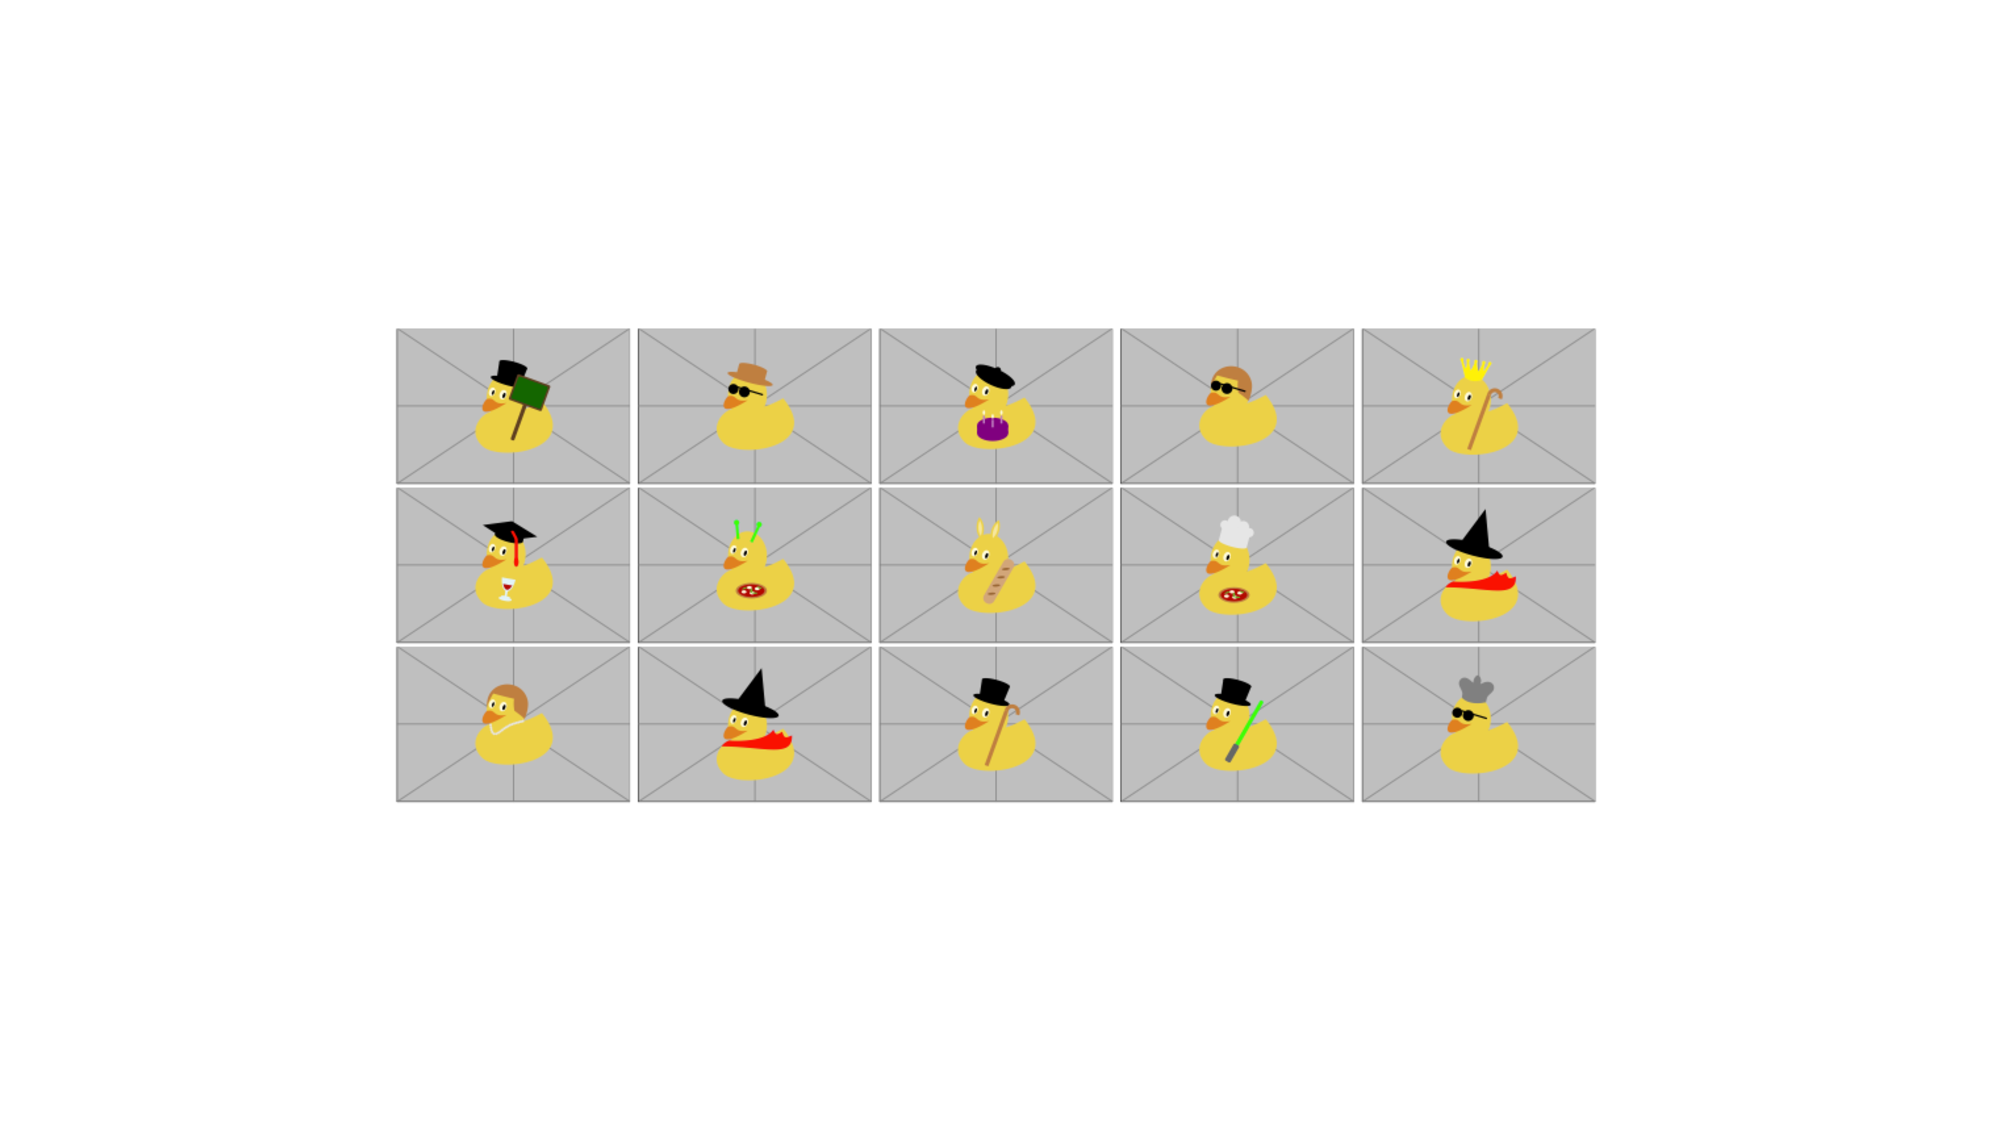
\includegraphics[width=\textwidth, trim={6cm 5cm 6cm 5cm},clip,page=1] {figures.pdf}
    \caption{Here are some photos of ducks to make you feel happy in tough times.}
    \label{fig:ducks}
\end{center}
\end{figure}



%%%%%%%%%%%%%%%%%%%%%%%%%%%%%%%%%%%%%%%%%%%%%%%%%%%%%%%%%%%%%%%%%%%%%%%%%%
%% for subsections and subsubsection, I did not like having numbered 
%% environmentsbecause it appeared confusing with my objectives and task 
%% numbering. so I used unnumbered subsections and subsubsections and added 
%% them to the table of content using \phantomsection and \addcontentsline 
%% commands before and after the corresponding environment.
%%%%%%%%%%%%%%%%%%%%%%% METHODOLOGY AND RESULTS %%%%%%%%%%%%%%%%%%%%%%%%%%

\section{Research objectives}                   %%% 1 page limit

\blindtext

%% 
\phantomsection
\subsection*{Objective 1: Some major objective here}
\addcontentsline{toc}{subsection}{Objective 1: Some major objective here}

\blindtext


%% add more objectives (one objective is not enough you know it)





%%%%%%%%%%%%%%%%%%%%%%%%%%%%%%%%%%%%%%%%%%%%%%%%%%%%%%%%%%%%%%%%%%%%%%%%%%
%% for subsections and subsubsection, I did not like having numbered 
%% environmentsbecause it appeared confusing with my objectives and task 
%% numbering. so I used unnumbered subsections and subsubsections and added 
%% them to the table of content using \phantomsection and \addcontentsline 
%% commands before and after the corresponding environment.
%%%%%%%%%%%%%%%%%%%%%%% METHODOLOGY AND RESULTS %%%%%%%%%%%%%%%%%%%%%%%%%%

\section{Proposed methodology and results}      %%% 4 page limit

\blindtext

\subsection{Task 1: Major project task heading here related to objective 1}

\blindtext


\phantomsection
\subsubsection*{Subtask 1.1: Some sub-task here}
\addcontentsline{toc}{subsubsection}{Subtask 1.1: Some sub-task here}

\blindtext




\subsubsection*{Subtask 1.2: Some other sub-task here}
\addcontentsline{toc}{subsubsection}{Subtask 1.2: Some other sub-task here}

\blindtext




%% add more tasks and subtasks (one task is not enough for PhD - you know it by now)





%%%%%%%%%%%%%%%%%%%%%%%%%%%%%% PUBLICATIONS %%%%%%%%%%%%%%%%%%%%%%%%%%%%%

\section{Planned publications}

\begin{enumerate} [leftmargin=0.75cm,itemsep=0pt]
    \item \fullcite{einstein}.
    \item \fullcite{knuth-fa}. \hfill (In preparation)
    %% add more items (if you have published/ planned for more papers)
\end{enumerate}





%%%%%%%%%%%%%%%%%%%%%%%%%%%%%%% TIMELINE %%%%%%%%%%%%%%%%%%%%%%%%%%%%%%%

\section{Timeline}

%% this is an example how to draw something using TikZ
%% I used a Timeline chart made using Excel/ PowerPoint combination
\begingroup
\begin{tikzpicture}
    % draw horizontal line   
    \draw[thick, -Triangle] (0,0) -- (\textwidth,0) node[font=\scriptsize,below left=3pt and -8pt]{years};
    
    % draw vertical lines
    \foreach \x in {0,1,...,10}
    \draw (\x cm,3pt) -- (\x cm,-3pt);
    
    \foreach \x/\descr in {4/t-2,5/t-1,6/t,7/t+1}
    \node[font=\scriptsize, text height=1.75ex,
    text depth=.5ex] at (\x,-.3) {$\descr$};
    
    % colored bar up
    \foreach \x/\perccol in
    {1/100,2/75,3/25,4/0}
    \draw[lightgray!\perccol!red, line width=4pt] 
    (\x,.5) -- +(1,0);
    \draw[-Triangle, dashed, red] (5,.5) --  +(1,0);
    
    % colored bar down
    \foreach \x/\perccol in
    {3/100,4/75,5/0}
    \draw[lightgray!\perccol!green, line width=4pt] 
    (\x,-.7) -- +(1,0);
    \draw[-Triangle, dashed, green] (6,-.7) --  +(1,0);
    
    % braces
    \draw [thick ,decorate,decoration={brace,amplitude=5pt}] (4,0.7)  -- +(2,0) 
           node [black,midway,above=4pt, font=\scriptsize] {Training period};
    \draw [thick,decorate,decoration={brace,amplitude=5pt}] (6,-.9) -- +(-1,0)
           node [black,midway,font=\scriptsize, below=4pt] {Testing period};
\end{tikzpicture}
\captionof{figure}{An abstract timeline to finish my PhD.}
\endgroup

%%%%%%%%%%%%%%%%%%%%%%%%%%%%% ACKNOWLEDGEMENT %%%%%%%%%%%%%%%%%%%%%%%%%%%%

%% Optional acknowledgment section (uncomment if you want to use)
\section*{Acknowledgement}
\addcontentsline{toc}{section}{Acknowledgement}

%% acknowledge your mentor, collaborators, and labmates if they helped you crafting your proposal or primary studies.
\blindtext


%%%%%%%%%%%%%%%%%%%%%%%%%%%%% BIBLIOGRAPHY %%%%%%%%%%%%%%%%%%%%%%%%%%%

\newpage
\section*{References}
\addcontentsline{toc}{section}{References}
\printbibliography[heading=none] 


%%%%%%%%%%%%%%%%%%%%%%%%%%% END BIBLIOGRAPHY %%%%%%%%%%%%%%%%%%%%%%%%%


%%%%%%%%%%%%%%%%%%%%%%%%%%%% END MAIN TEXT %%%%%%%%%%%%%%%%%%%%%%%%%%%


\end{document}

%%%%%%%%%%%%%%%%%%%%%%%%%%%% END DOCUMENT %%%%%%%%%%%%%%%%%%%%%%%%%%%%